\documentclass{article}

\usepackage[T1]{fontenc}
\usepackage[utf8]{inputenc}
\usepackage[greek,english]{babel}
\usepackage[a4paper, margin=0.2in]{geometry}
\usepackage{CJKutf8}

\usepackage{tikz}
\usepackage{float}
\usetikzlibrary{arrows}

\begin{document}
\begin{CJK}{UTF8}{gbsn}

\title{hw3}
\author{刘本嵩 U201614531}

\maketitle

% \foreignlanguage{greek}{φΔδ} \begin{CJK}{UTF8}{gbsn}汉\end{CJK}

\section{Q5.8}
\Large
\smallskip

(1) 总平均CPI = BaseCPI + 15\% * 分支指令的ExtraCPI

$$ExtraCPI = (90\% \dot 10\% \dot 4 + 10\% \dot 3) = 0.66$$

$$CPI = BaseCPI + 15\% ExtraCPI = 1.099$$

(2) 采用固定两个周期的开销, 即 $ExtraCPI = 2$

$$CPI = BaseCPI + 15\% ExtraCPI = 1.3$$

因此, 使用动态分支预测更好.

\section{Q5.9}
\Large
\smallskip

没有BTB时

$$CPI = 1.1 = 1 + 5\% \dot ExtraLatency$$

知无条件转移$ExtraLatency=2$. 因此有BTB的CPI为

$$CPI = 1 + 5\% \dot ExtraLatency \dot 10\% = 1.01$$

\section{Q5.11}
\Large
\smallskip

\begin{figure}[H]
\centering
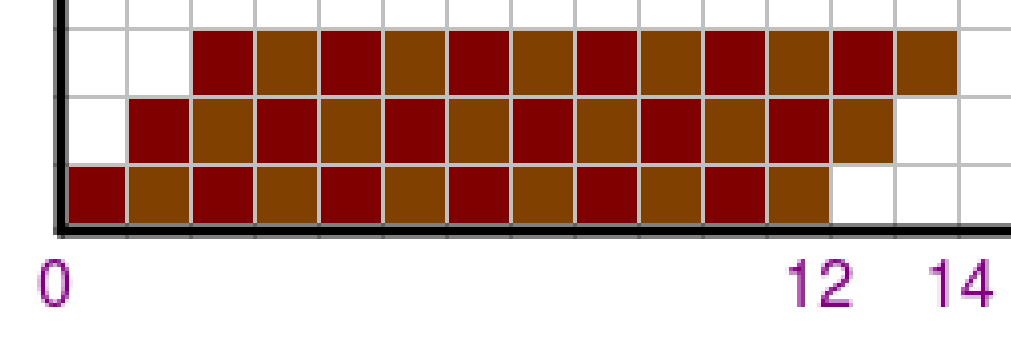
\includegraphics[scale=0.3]{hw3-img1.png}
\caption{标量流水 时空图}
\end{figure}

显然,标量流水一共使用$14\Delta t$

\begin{figure}[H]
\centering
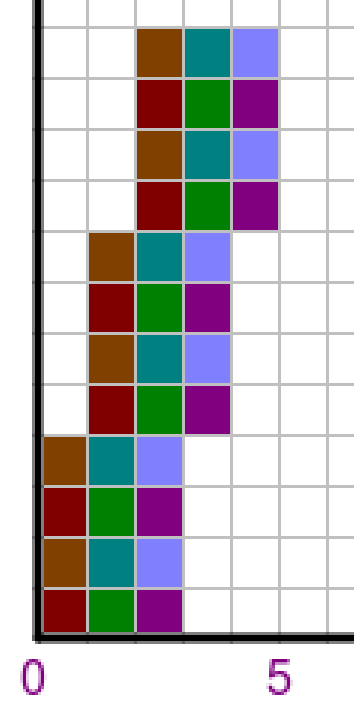
\includegraphics[scale=0.3]{hw3-img2.png}
\caption{超标量处理机 时空图}
\end{figure}

超标量处理机共使用$5\Delta t$, 加速比

$$SpeedUp = \frac{14\Delta t}{5\Delta t} = 2.8$$

\begin{figure}[H]
\centering
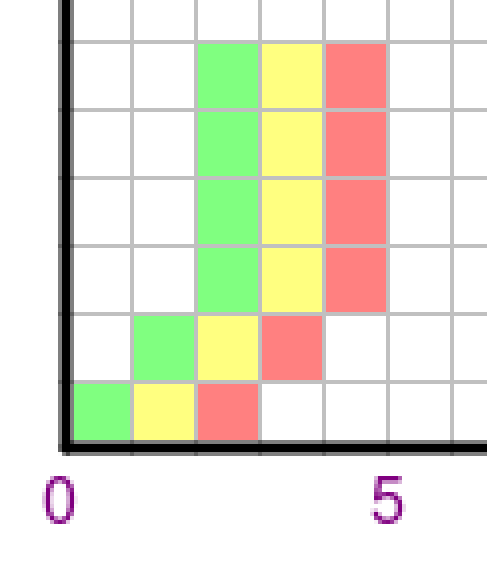
\includegraphics[scale=0.3]{hw3-img3.png}
\caption{超长指令处理机 时空图}
\end{figure}

超长指令处理机共使用$5\Delta t$, 加速比

$$SpeedUp = \frac{14\Delta t}{5\Delta t} = 2.8$$

\begin{figure}[H]
\centering
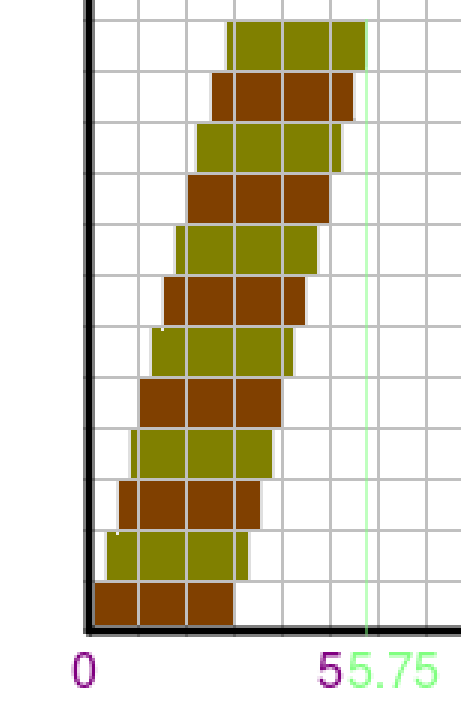
\includegraphics[scale=0.3]{hw3-img4.png}
\caption{超流水处理机 时空图}
\end{figure}

超流水处理机共使用$5.75\Delta t$, 加速比

$$SpeedUp = \frac{14\Delta t}{5.75\Delta t} = 2.435$$




\end{CJK}
\end{document}

